%%
% The BIThesis Template for Bachelor Graduation Thesis
%
% 北京理工大学毕业设计(论文)第一章节 —— 使用 XeLaTeX 编译
%
% Copyright 2020 Spencer Woo
%
% This work may be distributed and/or modified under the
% conditions of the LaTeX Project Public License, either version 1.3
% of this license or (at your option) any later version.
% The latest version of this license is in
%   http://www.latex-project.org/lppl.txt
% and version 1.3 or later is part of all distributions of LaTeX
% version 2005/12/01 or later.
%
% This work has the LPPL maintenance status maintained'.
%
% The Current Maintainer of this work is Spencer Woo.
%
% 第四章节
\chapter{基于GeoHash的矢量地图展现}
LeafLet\cite{leafletweb}是用于地图的开源JavaScript库之一,它是B / S端WebGIS开发项目中广泛使用的开源软件。开发人员可以基于相关库提供的接口进行开发和扩展,并实现地理信息服务的调用和地图数据的基本操作\cite{edler2019simplicity}。

Leaflet强大的开源库插件涉及地图应用程序的各个方面,包括地图服务,数据提供,数据格式,地理编码,路线搜索,地图控制和交互等,并且还支持自定义控件的实现。这些控件丰富了Leaflet的功能\cite{brambilla2016adgt}。GeoHashTile是基于轻量级的WebGIS库Leaflet来完成GeoHash编码地图数据展现的功能的。

基于地理信息的应用程序,例如导航服务和电子出租车服务为日常生活提供了极大的便利并促进了个人移动设备的普及\cite{li2018bringing},为了获得更好的用户体验,有必要提高访问速度,同时确保有效信息的保留。在“访问速度”和视觉效果之间找到最佳的方法是通过划分、索引和压缩大型地图数据来减少数据传输和提高效率。在大多数文献中,传输的数据元素是携带经纬度坐标的矢量地图数据,如果使用一维字符代表经纬度,这是减少传输数据量的可行方法;另外,对于大多数平铺地图,网络空间索引是被认为是对大量数据访问的有效改进方法,但是,网络空间索引使用三字段查询,这使得在大量数据访问的情况下效率十分低下,第三,数据压缩的数据不会显著降低视觉效果,同时量化方法通过减少位数来压缩数据和实值坐标的精度,可以保持对象的拓扑关系,但是,当实现良好的视觉效果时,如何选择合理的数据量化尺度是一个亟待解决的问题\cite{lawder2000using}。为此,GeoHashTile很好的解决了此类问题。

\section{GeoHashTile简介}
GeoHashTile是基于GeoHash编码的地图数据显示方法,改进了传统地理数据显示在数据索引,数据压缩,以及不同粒度的预测\cite{zhou2020geohashtile}。在此系统中,它使用Geohash编码系统代表坐标,并以此对大型地理数据进行分区和索引,数据压缩和图块编码也由GeoHash完成;它同时采用相对位置投影方法实现在GeoHash和屏幕像素坐标之间的直接转换,最后使用中间结果缓存的方法来提高计算和渲染效率。
\section{GeoHashTile架构}
GeoHashTile系统由两部分组成:服务器端和客户端,服务端提供矢量地理数据服务,客户端完成GeoHash矢量地理数据的显示,包括GeoHashTile计算过程,服务器地图数据的请求过程,GeoHash地图数据的投影过程以及中间结果缓存过程\cite{zhou2020geohashtile}。该功能框架如下:

服务器的工作分为两部分:Geohash矢量地理数据转换和Geohash矢量地理数据服务。数据转换中,将原始GeoJSON数据集的纬度和经度坐标转换为相对应的指定长度的Geohash编码的GeoJSON格式数据,并将数据重新组织为GeoJSON格式数据以供客户端访问,该数据还定义了数据访问接口并设置数据精度。收到客户端发送的HTTP请求后,数据服务部分将分解字段,查询相应的Geohash编码的GeoJSON数据,并通过HTTP响应将其返回给客户端,其中Geohash编码的矢量地理数据服务由GeoServer提供-基于Web的服务器。

客户端工作分为四个部分:
\begin{enumerate}
    \item GeoHashTile计算部分,计算一块GeoHashTile的大小,计算客户端中GeoHashTile的数量,以及计算客户端中所有GeoHashTile编码
    \item 接收地图数据
    \item 通过相对位置投影的方法,实现屏幕像素点到GeoHash坐标值的转换
    \item 通过中间结果缓存来减少重复计算处理,加快图像的呈现
\end{enumerate}

\section{GeoHashTile优点}
GeoHashTile以减少数据传输,提高索引效率和减少加载时间的目标出发,研究了基于GeoHash的矢量地理数据结构,同时提出了地图数据的GeoHashTile系统索引,实现了GeoHash坐标编码的地图数据展示。GeoHashTile系统在减少用户的等待时间的同时不会影响显示效果,它使应用程序减少了数据传输和加载时间,它还提供了支持GeoHash编码的新矢量数据服务,实验结果表明,在减少数据量方面,由于GeoHash压缩了经纬度,不同级别的不同粒度地图数据的存储以及数据合并访问,因此GeoHashTile的平均表现要比GeoTile优43.7\%,web客户端上GeoHashTile的加载时间也比GeoTile短30.2\%。

\section{总体测试框架和运行环境}
\subsection{测试环境}
本次测试,使用nvm-v0.37.2管理nodejs版本,使用npm-v6.14.11包管理,智能合约语言使用Solidty-v0.5.16,在前端调用合约方法上,使用web3js-v1.2.9与之进行交互。在对合约 进行测试时,采用ganache-cli提供本地临时区块链私有链服务,并使用Truffle-v5.1.62辅助部署智能合约,简化了开发和测试流程。在正式应用上,采用geth-v1.9.12以太坊客户端,部署本地私有链,存储相关信息。因为本文应用均是基于最新的开发环境,在编写合约和测试过程中遇到过很多问题,因此编写了许多有关环境配置以及简单示例文件的相关帮助手册,希望能为其他人提供帮助。

\subsection{测试流程}
为了验证地图存储的正确性,本文将此工作与前人相关工作合并,使用GeoHashTile前端对地图数据进行展示。

随着区块链的普遍应用,对应平台也逐渐增多,主流平台还是以太坊。此测试也是在该平台进行相关操作,总体测试流程如下:

\begin{enumerate}
    \item 首先建立Geth私有链;
    \item 通过truffle工具可以简单部署合约到区块链上;
    \item 通过JS脚本将地图数据进行上传及绑定;
    \item 由于时间原因,该测试只是为了验证地图存储的正确性,所以仅上传部分北京数据,并使用GeoHashTile前端对其信息进行展示,结果如图\ref{GeoHashTile展示结果}GeoHashTile展示结果,\ref{放大图}放大图,\ref{缩小图}缩小图。
    \begin{figure}[!htb]
        \centering
        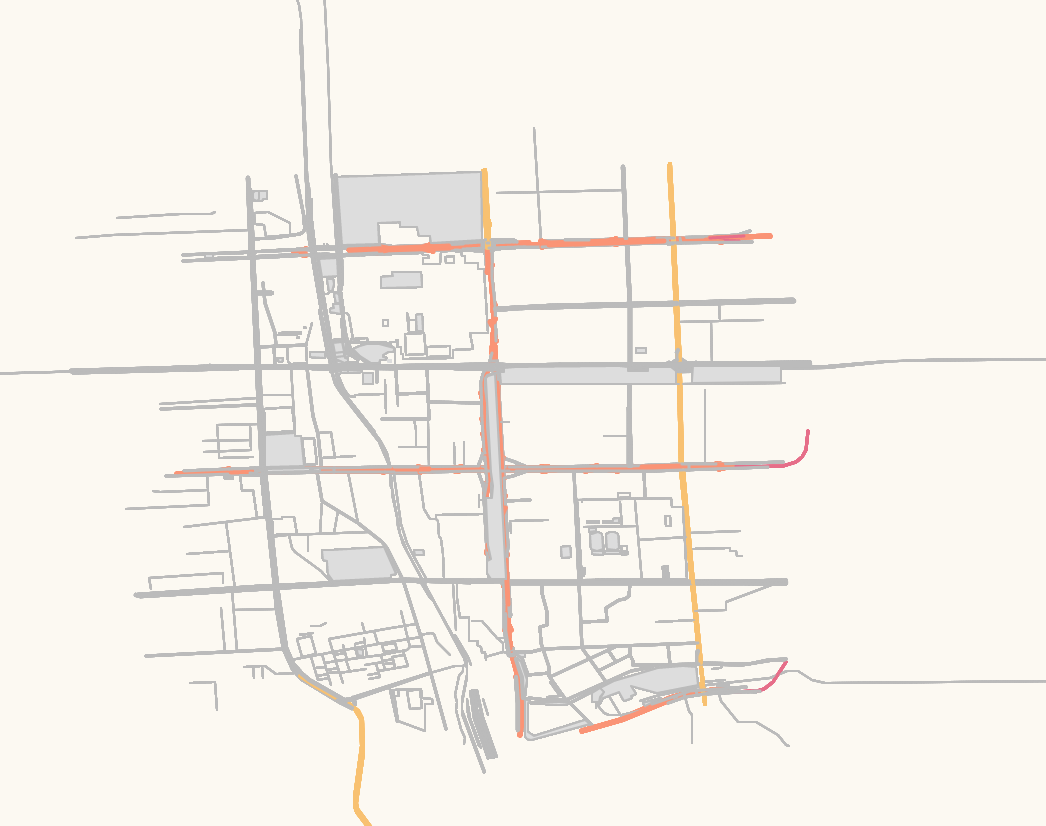
\includegraphics[width=4in]{images/6.png}
        \caption{GeoHashTile展示结果}\label{GeoHashTile展示结果} % label 用来在文中索引
    \end{figure}

    \begin{figure}[!htb]
        \centering
        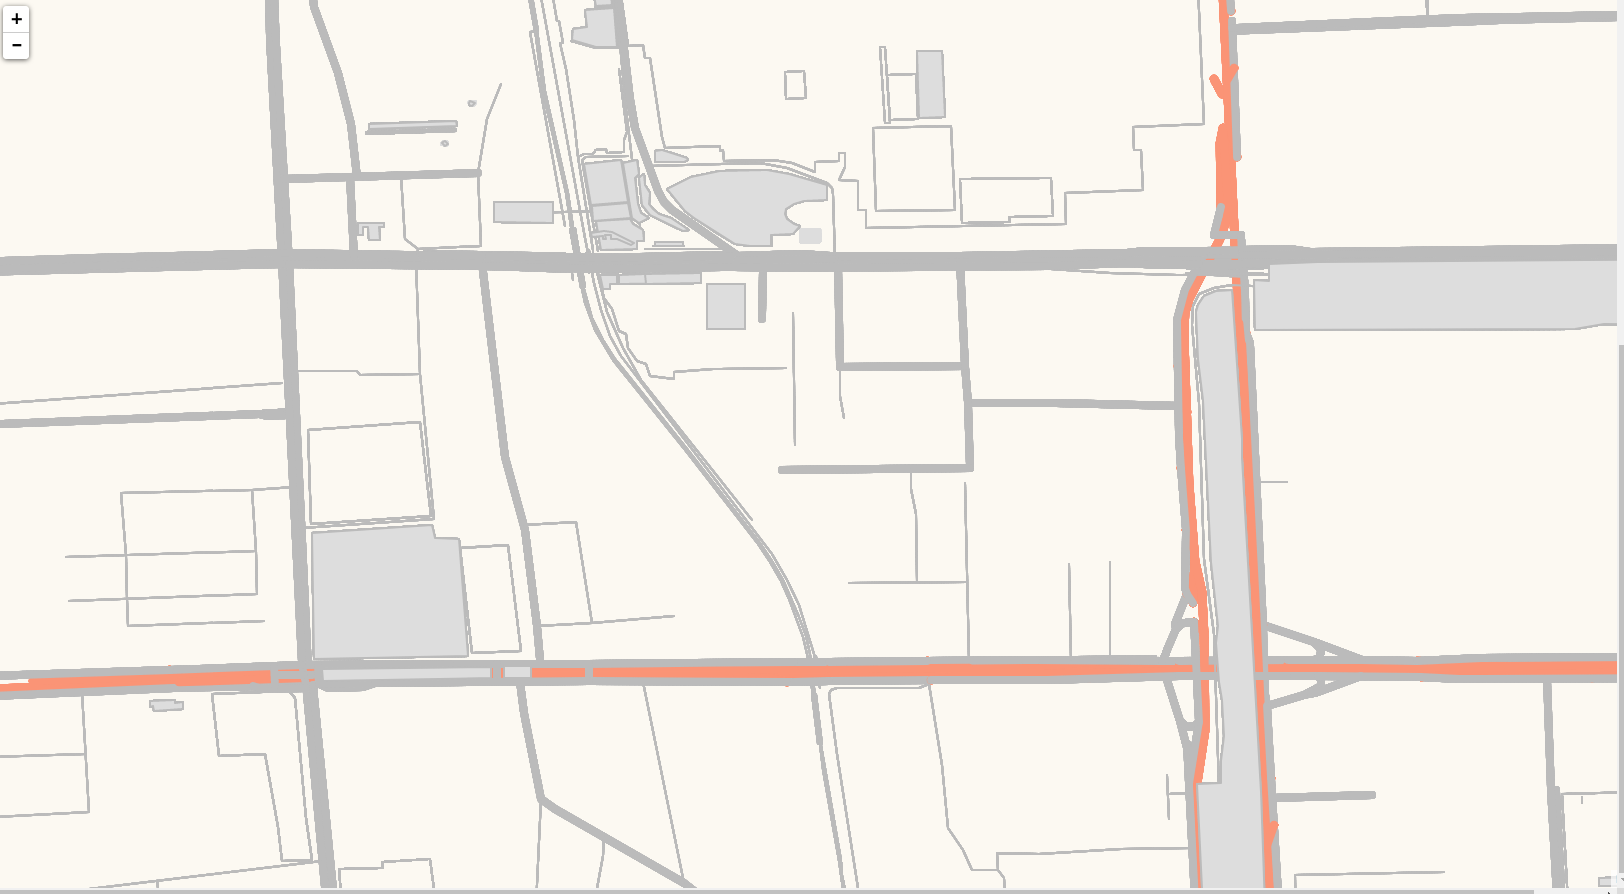
\includegraphics[width=4in]{images/11.png}
        \caption{放大图}\label{放大图} % label 用来在文中索引
    \end{figure}

    \begin{figure}[!htb]
        \centering
        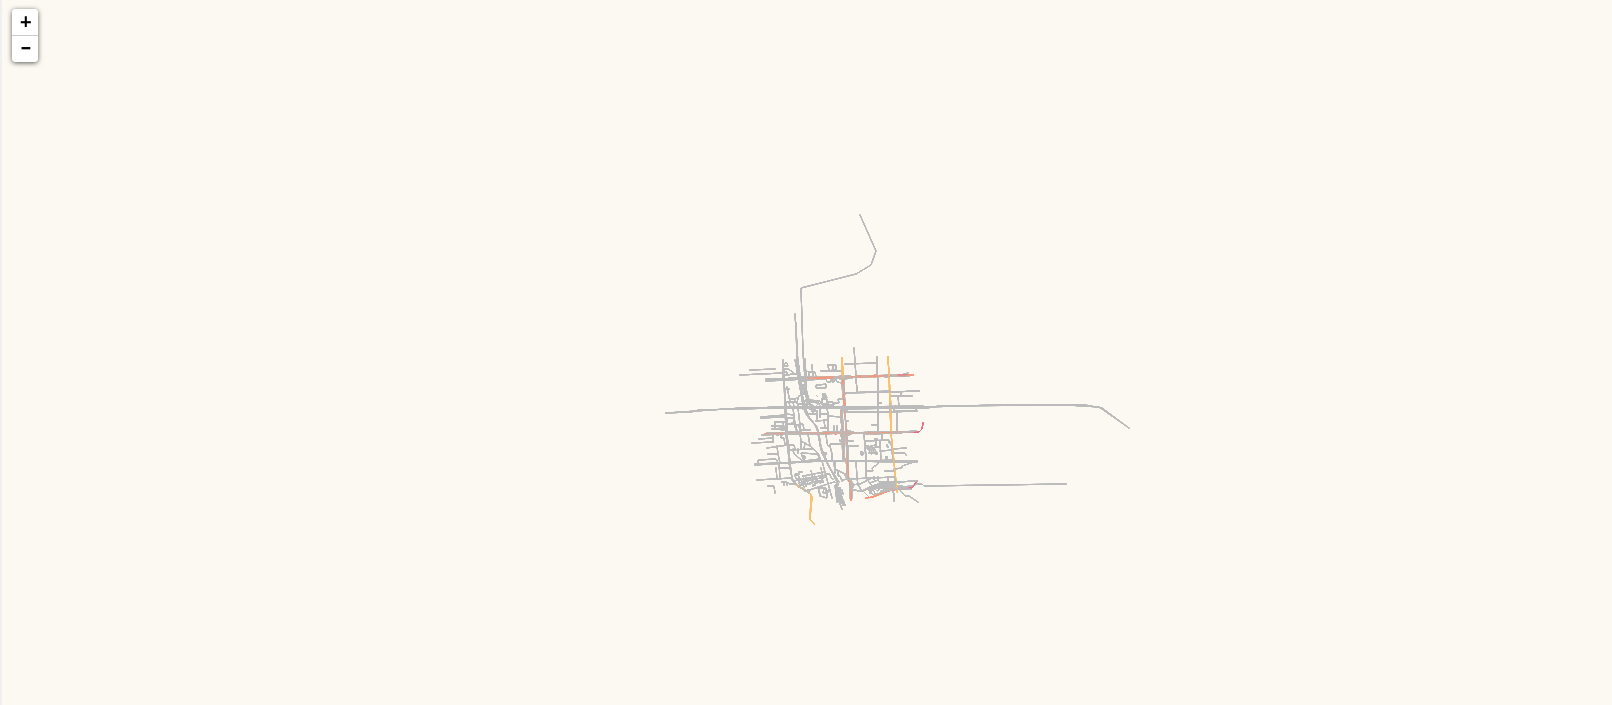
\includegraphics[width=4in]{images/12.png}
        \caption{缩小图}\label{缩小图} % label 用来在文中索引
    \end{figure}
\end{enumerate}

\section{小结}
GeoHash编码使用一维数据替代了二维经纬度数据,同时给地理位置进行了分区,在位数较少时,它可以用来表示某一区域在地球上的坐标,在位数足够时,它也可以用来表示某个具体点在地球上的坐标。在 GeoHash 精度取 8 位的情况下已经可以基本满足代替传统经纬度坐标作为车辆位置精确表示的需求,且若只考虑中国所处纬度(3°51′N 至53°33′N),精度将会提高\cite{lposition}。考虑到车辆位置验证以及道路匹配需要更高的精准度,所以之后的工作中采用了11位长度的GeoHash编码。

GeoHashTile提高了矢量地图的索引效率和加载时间,且提供了支持GeoHash编码的新矢量数据服务。

测试表明,目前该系统可以成功将地图数据经纬度格式转为GeoHash格式,并上传到以太坊私链进行保存,且能够通过GeoHashTile可以正确显示GeoHash矢量数据。